\documentclass[a4paper]{article}
\usepackage{times}
\usepackage[utf8]{inputenc}
\usepackage{selinput}
\usepackage{upquote}
\usepackage[margin=2cm, rmargin=4cm, tmargin=3cm]{geometry}
\usepackage{tcolorbox}
\usepackage{xspace}
\usepackage[french]{babel}
\usepackage{url}
\usepackage{hyperref}
\usepackage{fontawesome5}
\usepackage{marginnote}
\usepackage{ulem}
\usepackage{tcolorbox}
\usepackage{graphicx}
%\usepackage[top=Bcm, bottom=Hcm, outer=Ccm, inner=Acm, heightrounded, marginparwidth=Ecm, marginparsep=Dcm]{geometry}


\newtcolorbox{Example}[1]{colback=white,left=20pt,colframe=slideblue,fonttitle=\bfseries,title=#1}
\newtcolorbox{Solutions}[1]{colback=white,left=20pt,colframe=green,fonttitle=\bfseries,title=#1}
\newtcolorbox{Conseils}[1]{colback=white,left=20pt,colframe=slideblue,fonttitle=\bfseries,title=#1}
\newtcolorbox{Warning}[1]{colback=white,left=20pt,colframe=warning,fonttitle=\bfseries,title=#1}

\setlength\parindent{0pt}

  %Exercice environment
  \newcounter{exercice}
  \newenvironment{Exercice}[1][]
  {
  \par
  \stepcounter{exercice}\textbf{Question \arabic{exercice}:} (\faClock \enskip \textit{#1})
  }
  {\bigskip}
  

% Title
\newcommand{\titre}{\begin{center}
  \section*{Algorithmes et Pensée Computationnelle}
\end{center}}
\newcommand{\cours}[1]
{\begin{center} 
  \textit{#1}\\
\end{center}
  }


\newcommand{\exemple}[1]{\newline~\textbf{Exemple :} #1}
%\newcommand{\attention}[1]{\newline\faExclamationTriangle~\textbf{Attention :} #1}

% Documentation url (escape \# in the TP document)
\newcommand{\documentation}[1]{\faBookOpen~Documentation : \href{#1}{#1}}

% Clef API
\newcommand{\apikey}[1]{\faKey~Clé API : \lstinline{#1}}
\newcommand{\apiendpoint}[1]{\faGlobe~Url de base de l'API \href{#1}{#1}}

%Listing Python style
\usepackage{color}
\definecolor{slideblue}{RGB}{33,131,189}
\definecolor{green}{RGB}{0,190,100}
\definecolor{blue}{RGB}{121,142,213}
\definecolor{grey}{RGB}{120,120,120}
\definecolor{warning}{RGB}{235,186,1}

\usepackage{listings}
\lstdefinelanguage{texte}{
    keywordstyle=\color{black},
    numbers=none,
    frame=none,
    literate=
           {é}{{\'e}}1
           {è}{{\`e}}1
           {ê}{{\^e}}1
           {à}{{\`a}}1
           {â}{{\^a}}1
           {ù}{{\`u}}1
           {ü}{{\"u}}1
           {î}{{\^i}}1
           {ï}{{\"i}}1
           {ë}{{\"e}}1
           {Ç}{{\,C}}1
           {ç}{{\,c}}1,
    columns=fullflexible,keepspaces,
	breaklines=true,
	breakatwhitespace=true,
}
\lstset{
    language=Python,
	basicstyle=\bfseries\footnotesize,
	breaklines=true,
	breakatwhitespace=true,
	commentstyle=\color{grey},
	stringstyle=\color{slideblue},
  keywordstyle=\color{slideblue},
	morekeywords={with, as, True, False, Float, join, None, main, argparse, self, sort, __eq__, __add__, __ne__, __radd__, __del__, __ge__, __gt__, split, os, endswith, is_file, scandir, @classmethod},
	deletekeywords={id},
	showspaces=false,
	showstringspaces=false,
	columns=fullflexible,keepspaces,
	literate=
           {é}{{\'e}}1
           {è}{{\`e}}1
           {ê}{{\^e}}1
           {à}{{\`a}}1
           {â}{{\^a}}1
           {ù}{{\`u}}1
           {ü}{{\"u}}1
           {î}{{\^i}}1
           {ï}{{\"i}}1
           {ë}{{\"e}}1
           {Ç}{{\,C}}1
           {ç}{{\,c}}1,
    numbers=left,
}

\newtcbox{\mybox}{nobeforeafter,colframe=white,colback=slideblue,boxrule=0.5pt,arc=1.5pt, boxsep=0pt,left=2pt,right=2pt,top=2pt,bottom=2pt,tcbox raise base}
\newcommand{\projet}{\mybox{\textcolor{white}{\small projet}}\xspace}
\newcommand{\optionnel}{\mybox{\textcolor{white}{\small Optionnel}}\xspace}
\newcommand{\advanced}{\mybox{\textcolor{white}{\small Pour aller plus loin}}\xspace}
\newcommand{\auto}{\mybox{\textcolor{white}{\small Auto-évaluation}}\xspace}


\usepackage{environ}
\newif\ifShowSolution
\NewEnviron{solution}{
  \ifShowSolution
	\begin{Solutions}{\faTerminal \enskip Solution}
		\BODY
	\end{Solutions}
  \fi}


  \usepackage{environ}
  \newif\ifShowConseil
  \NewEnviron{conseil}{
    \ifShowConseil
    \begin{Conseils}{\faLightbulb \quad Conseil}
      \BODY
    \end{Conseils}

    \fi}

    \usepackage{environ}
  \newif\ifShowWarning
  \NewEnviron{attention}{
    \ifShowWarning
    \begin{Warning}{\faExclamationTriangle \quad Attention}
      \BODY
    \end{Warning}

    \fi}
  

%\newcommand{\Conseil}[1]{\ifShowIndice\ \newline\faLightbulb[regular]~#1\fi}



\usepackage{array}
\newcolumntype{C}[1]{>{\centering\let\newline\\\arraybackslash\hspace{0pt}}m{#1}}

\begin{document}

% Change the following values to true to show the solutions or/and the hints
\ShowSolutiontrue
\ShowConseiltrue
\titre
\cours{Algorithmes de graphes}

Le but de cette séance est de comprendre le fonctionnement des graphes et d'appliquer des algorithmes courants sur des graphes simples. \\
\begin{note}{"Nathan"}
    q1-7: basique (temps raisonnable et mise à part les exos 1 et 4 niveau d'abstraction bas)
    q7-16: basique
    q8,9: avancé 
\end{note}
\section{Breadth-First Search}

\begin{Exercice}[5 minutes]  \textbf{Adjacency list et adjacency matrix : Python}\\
    L'adjacency list (ou liste de contiguïté) et l'adjacency matrix (ou matrice de contiguïté) sont les 2 méthodes dont nous disposons pour représenter un graphe. Utilisez ces 2 méthodes de représentations pour stocker le graphe ci-dessous dans un programme Python :\\
    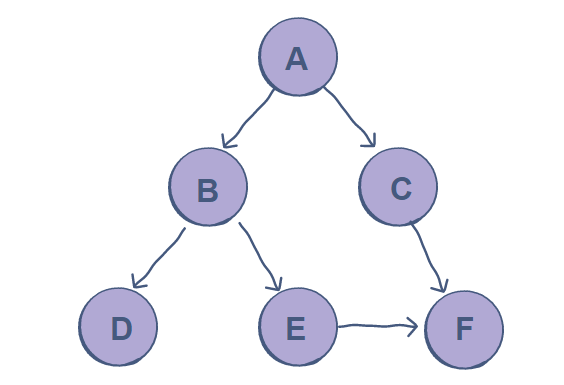
\includegraphics[]{Graphe1.PNG}   

    \begin{conseil}
    Pour l'adjacency list, utilisez un dictionnaire Python. Pour l'adjacency matrix, utilisez une liste multidimensionnelle (ou liste contenant une ou plusieurs listes).
    \end{conseil}
    \begin{solution}
        \lstinputlisting[language=python]{Question1_solution.py}
        Le fait que le graphe soit dirigé joue un rôle important pour la construction de ces représentations. Par exemple, pour l'adjacency list, 'B' apparaît dans la liste correspondant à la clé 'A' mais l'inverse n'est pas vrai. Cela signifie que l'on peut aller du sommet A au sommet B mais pas du sommet B au sommet A.\\
    \end{solution}
\end{Exercice}


\begin{Exercice}[15 minutes]  \textbf{Breadth-First Search algorithm : Python}\\
    Nous allons maintenant nous intéresser au premier algorithme portant sur les graphes : \textbf{Breadth-First search}. Le but du Breadth-first search est de trouver tout les sommets atteignables à partir d'un sommet de départ.\\
    Implémentez l'algorithme en suivant les étapes suivantes :\\
    \begin{enumerate}
    
    \item Partez du sommet initial, visitez les sommets adjacents, sauvegardez-les comme \textbf{visités}, insérez-les dans une \textbf{queue}.
    
    \item Parcourez la \textbf{queue}. Pour chaque élément de la queue, visitez les sommets adjacents. S'ils ne sont pas dans la liste des sommets visités, ajoutez-le à cette dernière et ajoutez-le à la queue. Une fois que cela est fait, supprimez l'élément parcouru de la queue.
    
    \item Répétez l'étape 2 jusqu'à ce que la queue soit vide.\\

    \end{enumerate}

    \begin{conseil}
        Quelques conseils pour l'implémentation de votre algorithme :
        \begin{enumerate}
            \item Utilisez l'adjacency list.
            \item Pour le point 3), utilisez une boucle \lstinline{while} avec la condition appropriée.
            \item Pour parcourir les sommets adjacents, utilisez une boucle for .
            \item L'algorithme devrait retourner une liste contenant l'ensemble des sommets atteignables.
            \item Vous pouvez utiliser l'image du graphe pour déterminer si l'output de votre l'algorithme est correct.
        \end{enumerate}
    \end{conseil}
    \begin{solution}
        \lstinputlisting[language=python]{Question2_solution.py}
        Si vous avez correctement codé votre algorithme, l'output de celui-ci avec comme input notre graphe et le sommet 'A' devrait être ['A', 'B', 'C', 'F', 'D', 'E']
    \end{solution}
\end{Exercice}

\newpage

\section{Minimum Spanning tree}
    Nous allons maintenant nous intéresser à \textbf{l'algorithme de Kruskal}. Ce dernier s'applique uniquement aux \textbf{weighted graphs}~(ou graphes pondérés). Ces derniers sont des graphes où les arêtes ont des poids, représentant par exemple une distance. L'algorithme de Kruskal a pour but de trouver un \textbf{minimum spanning tree}. Un minimum spanning tree S de G est un sous-graphe connexe de G tel que :
    \begin{enumerate}
        \item V' = V, c'est-à-dire que tous les sommets de G sont aussi dans S
        \item (V',E') ne contient pas de cycle (pas de cycle dans S)
        \item S est le graphe satisfaisant 1) et 2) et ayant la plus petite somme des poids
    \end{enumerate}
    
    \textbf{\\}

\begin{Exercice}[5 minutes] \textbf{Algorithme de Kruskal : Papier}\\
    Appliquez l'algorithme de Kruskal au graphe suivant :\\
    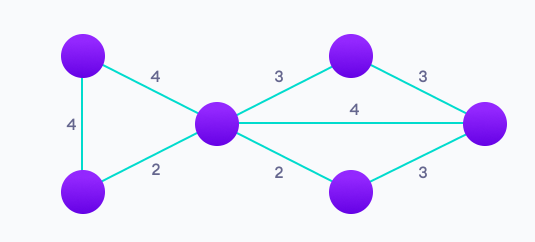
\includegraphics[]{Kruskal.PNG}
    \begin{conseil}
        L'algorithme de Kruskal fonctionne de la façon suivante :
        \begin{enumerate}
            \item Classer les arêtes par ordre croissant de poids.
            \item Prendre l'arête avec le poids le plus faible et l'ajouter à l'arbre (si 2 arêtes ont le même poids, choisir arbitrairement une des 2).
            \item Vérifiez que l'arête ajoutée ne crée pas de cycle, si c'est le cas, supprimez la.
            \item Répétez les étapes 2) et 3) jusqu'à ce que tous les sommets aient été atteints.
        \end{enumerate}
        Un Minimum Spanning Tree, s'il existe, a toujours un nombre d'arêtes égal au nombre de sommets moins un. Par exemple, ici notre graphe a 6 sommets. L'algorithme devrait donc s'arrêter lorsque 5 arêtes ont été choisies.
    \end{conseil}
    \begin{solution}
        Vous trouverez ci-dessous les étapes de la construction du MST(Minimum spanning tree) :\\
        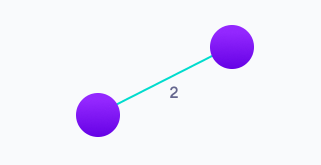
\includegraphics[]{K1.PNG}\\
        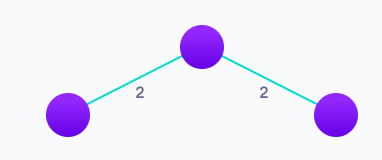
\includegraphics[]{K2.PNG}\\
        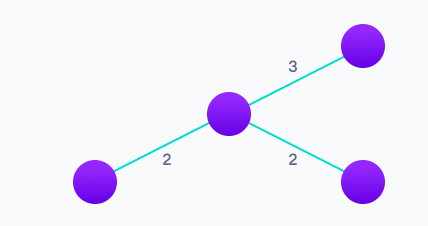
\includegraphics[]{K3.PNG}\\
    \end{solution}
    \begin{solution}
        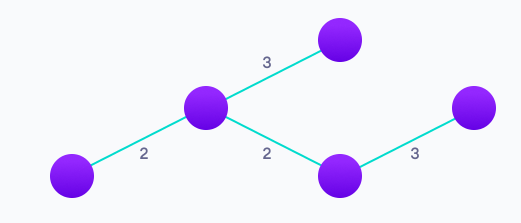
\includegraphics[]{K4.PNG}\\
        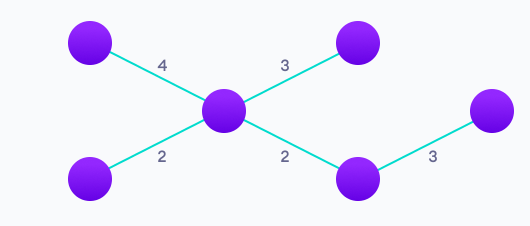
\includegraphics[]{K5.PNG}\\
        L'algorithme s'arrête car tous les sommets ont été atteints. On voit bien que seules 5 arêtes ont été nécessaire.
    \end{solution}
\end{Exercice}

\begin{note}{Maeva}
    Ceci devrait être un exercice avancé
\end{note}

\begin{Exercice}[15 minutes] \textbf{Algorithme de Kruskal : Python}\\
    Vous trouverez ci-dessous l'algorithme de Kruskal implémenté en Python. Parcourez la fonction \textbf{Kruskal\_algo(Graph)} afin de vous assurez que vous ayez bien compris le fonctionnement :\\
    \lstinputlisting[language=python]{Question3_solution.py}
    \begin{conseil}
        La partie \lstinline{class Graph} est une notion que vous verrez dans les chapitres dédiés à la programmation orientée objet. Pour le moment, il n'est pas important de comprendre son fonctionnement. L'output de l'algorithme est : \\
        1 - 2: 2\\
        2 - 5: 2\\
        2 - 3: 3\\
        3 - 4: 3\\
        0 - 1: 4\\
        Il se lit comme une liste d'arêtes et de poids à l'arête correspondante.
    \end{conseil}
\end{Exercice}

\newpage

\begin{note}{Maeva}
    Ceci devrait être un exercice avancé
\end{note}
\begin{Exercice}[10 minutes] \textbf{Social Network Analysis : Papier}\\
    Les graphes peuvent être utilisés pour représenter une multitude de choses.  L'une d'entre elles est la représentation de votre réseau d'amis. Imaginez que vous possédiez une liste de vos amis ainsi que des amis de vos amis (qui ne sont pas nécessairement vos amis). Cette liste peut-être représentée sous forme de graphe. Dans ce graphe :\\
    \begin{enumerate}
        \item  À quoi correspondent les arêtes et les nœuds ? 
        \item Faut-il utiliser un graphe dirigé ?
    \end{enumerate}
    Supposez que vous disposiez d'un graphe des relations sociales. Décrivez comment retrouver les éléments suivants :
    \begin{enumerate}
        \item Votre ami qui a le plus d'ami
        \item Découvrir quels amis à vous se connaissent
        \item Listez vos amis qui pourraient vous présenter quelqu'un que vous ne connaissez pas (ami d'ami qui n'est pas votre ami)
    \end{enumerate}
    Vous voudriez désormais ajouter une nouvelle personne sur ce graphe, mais cette dernière n'est ni votre ami, ni l'ami d'un de vos amis. Quel sera son degré dans le graphe ?\\
    
    Retrouvez les éléments 1) à 3) dans le graphe ci-dessous :\\
    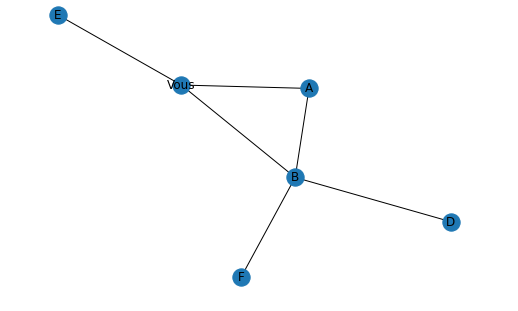
\includegraphics[]{Network1.PNG}
    \begin{conseil}
        Réfléchissez en terme d'arêtes, de sommets, de degrés et de cycles.
    \end{conseil}

    \begin{solution}
        Dans le graphe des relations sociales, les arêtes correspondent à un lien d'amitié et les nœuds représentent les personnes. Il n'est pas nécessaire d'utiliser un graphe dirigé si l'on considère qu'une relation d'amitié est toujours réciproque.\\
        
        Pour trouver les éléments 1) à 3), il faut raisonner de la façon suivante :
        \begin{enumerate}
            \item Trouvez le sommet relié à vous qui a le degré le plus élevé. Sommet B dans le graphe.
            \item Premièrement, les 2 personnes doivent être mes amis donc reliées à moi, mais de  plus elles doivent être reliées entre elles. Par conséquent, cela correspond à un cycle dans le graphe. Il y a autant d'amis qui se connaissent que de cycle dans le graphe. Ami A et B dans le graphe.
            \item Il ne doit pas y avoir d'arêtes me reliant avec l'ami de mon ami. Sommet B dans le graphe.
        \end{enumerate}
        
        Si l'on ajoute une personne qui n'est ni un ami, ni l'ami d'un ami, alors aucune arête n'est reliée à ce sommet. Par conséquent, ce sommet a un degré 0.
    \end{solution} 
\end{Exercice}

\begin{note}{Maeva}
    Ceci devrait être un exercice avancé
\end{note}
\begin{Exercice}[5 minutes] \textbf{Reconnaître des réseaux semblables}\\
    Supposons maintenant que vous travaillez chez Facebook, qui a récemment racheté Whatsapp et que vous disposiez des 2 graphes représentant respectivement Facebook et Whatsapp. Pouvez-vous déterminer à qui correspondent les individus de Facebook sur Whatsapp ?\\
    
    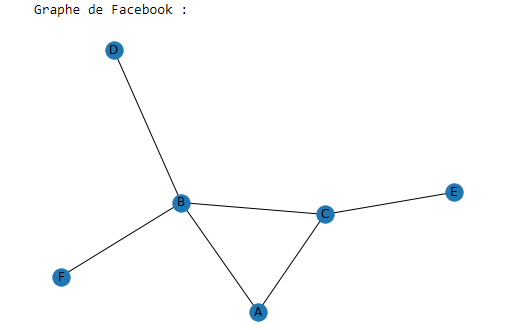
\includegraphics[]{Network2.PNG}\\
    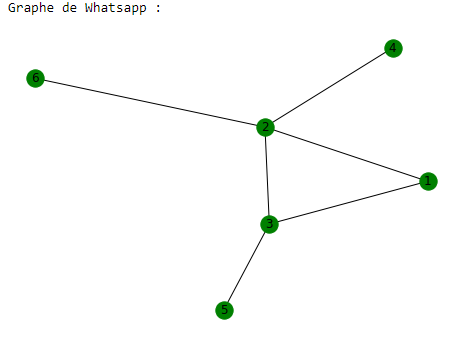
\includegraphics[]{Network3.PNG}
    
    
    \begin{conseil}
    Quelques hints pour vous aider à résoudre cet exercice :
    \begin{enumerate}
        \item Identifiez les sommets des 2 graphes avec des caractéristiques semblables.
        \item Il est possible que les sommets ne soient pas tous identifiables.
    \end{enumerate}
        
    \end{conseil}
    \begin{solution}
        \begin{enumerate}
            \item B correspond à 2 (seul sommet de degré 4)
            \item A correspond à 1 (seul sommet de degré 1 relié au sommet de degré 4)
            \item C correspond à 3 (seul sommet de degré 3)
            \item E correspond à 5 (seul sommet de degré 1 relié au sommet de degré 2)
        \end{enumerate}
        Les sommets D et F et 4 et 6 ne peuvent pas être dissociés. On ne peut donc pas savoir qui correspond à qui.
    \end{solution}
\end{Exercice}

\newpage


\section{Algorithme de Dijkstra : Python}
Nous allons nous intéresser à l'algorithme de Dijkstra qui permet de calculer le chemin le plus court entre 2 sommets d'un graphe. Cet algorithme est par exemple utilisé par les systèmes de navigation (GPS par exemple) pour trouver le chemin le plus court ou le moins coûteux entre 2 points. Les questions de cet exercice sont à remplir sur le fichier Exercice3.py disponible sur Moodle dans le dossier Ressources. \\
\begin{Exercice}[10 minutes]\textbf{Un petit échauffement}\\

Avant de rentrer dans le vif du sujet, nous allons devoir passer par quelques étapes préliminaires afin que vous puissiez coder l'algorithme par vous même. Considérez le graphe suivant :\\
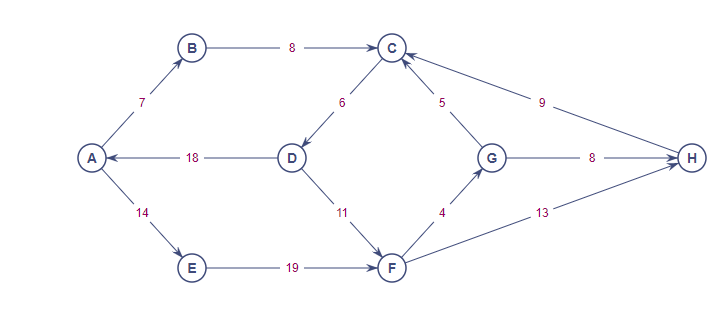
\includegraphics[]{Dijkstra.PNG}

Ouvrez le fichier Exercice3.py, et prenez connaissance du code, votre objectif sera de le compléter. Premièrement, représentez le graphe sous la forme d'une \lstinline{adjacency matrix}.
\end{Exercice}
\begin{conseil}
    Représentez la matrice avec les colonnes et les lignes par ordre alphabétique.
\end{conseil}
\begin{solution}
    \lstinputlisting[language=python]{Question7_solution.py}
\end{solution}
\newpage
\begin{Exercice}[10 minutes]\textbf{Des outils utiles}\\
    La première étape étant complétée, nous allons maintenant nous intéresser à comment récupérer des informations de notre graphe. Voici une liste non-exhaustive d'opérations que l'on peut effectuer :\\
    \begin{enumerate}
        \item get\_node() permet d'accéder à un nœud. Par exemple, en faisant graphe.get\_node('A'), j'obtiens des informations concernant le nœud A.
        \item Lorsque l'on accède à un nœud par la fonction get\_node(), on peut ensuite accéder à la liste de toutes les arêtes qui s'y connecte par l'attribut \lstinline{relationships}. On peut par la suite distinguer les arêtes partant du nœud et les arêtes y arrivant à l'aide des attributs \lstinline{relationship._from} et \lstinline{relationship.to}.
    \end{enumerate}
    
    L'exemple de code ci-dessous devrait vous aider à mieux comprendre :
    \lstinputlisting[language = python]{Question8_exemple.py}
    
    Pour vous assurez que vous avez bien compris cette partie avant de commencer, complétez la fonction linked du fichier Exercice3.py de sorte à ce que la fonction permette d'afficher tout les nœuds \textbf{partant} d'un sommet donné et d'afficher le poids de l'arête reliant ces 2 sommets.\\
    
    
    \begin{conseil}
        Quelques hints pour écrire ce programme :
        \begin{enumerate}
            \item Vous devrez retirez les sommets reliés par une arête avec un poids de 99999
            \item Utilisez une boucle for pour parcourir les arêtes
        \end{enumerate}
    Votre output devrait être A 18, F 11.
    \end{conseil}
    \begin{solution}
        \lstinputlisting[language = python]{Question8_solution.py}
    \end{solution}
\end{Exercice}
\newpage

\begin{note}{Maeva}
    Ceci devrait être un exercice avancé
\end{note}
\begin{Exercice}[15 minutes] \textbf{Algorithme de Dijkstra \optionnel}\\
    L'algorithme de Dijkstra permet de calculer le chemin le plus court entre 2 sommets d'un graphe.~L'algorithme~de~Dijkstra~que l'on va utiliser se construit de façon récursive. On initialise l'algorithme à partir du point de départ. Puis, l'on va se déplacer vers tous les sommets atteignables depuis notre point de départ et appliquer l'algorithme de Dijkstra à ses voisins. Ainsi de suite jusqu'à ce que l'on atteigne le sommet de destination. Pour éviter de créer une boucle infinie à cause des cycles, nous appliquerons uniquement Dijkstra aux voisins qui n'ont pas encore été visité.\\
    
    Complétez la fonction \lstinline{dijkstra} du fichier \lstinline{Exercice3.py}. Pour y arriver, vous pouvez suivre les étapes suivantes:
    \begin{enumerate}
        \item L'algorithme de Dijkstra est un algorithme récursif. Nous l'avons vu lors des dernières semaines, il est nécessaire d'avoir une condition d'arrêt. L'algorithme appelle la fonction \lstinline{dijkstra} de façon récursive en spécifiant l'origine (qui changera à chaque appel de la fonction \lstinline{dijkstra}) et la destination. Quelle condition semble appropriée pour terminer l'appel récursif ? Implémentez cette condition dans la partie \textbf{Question 9.1}
        
        \item Maintenant, nous allons avoir besoin d'une boucle parcourant toutes les relations voisines à notre point d'origine. Pour rappel, \textit{origin.relationships} donne la liste des relations (sommet d'arrivée et poids de l'arête) à partir d'un sommet de départ. Implémentez cette boucle dans la partie \textbf{Question 9.2}.
        
        \item À présent, nous pouvons sauter certaines itérations. Pour rappel, nous avons utilisé une matrice d'adjacence pour représenter notre graphe. Mais certaines relations ont vu leur poids arbitrairement assigné à 99999, pour signifier que 2 sommets n'étaient pas reliés. Implémentez une condition qui permet de passer à l'itération suivante de la boucle dans le cas où le poids de l'arête entre l'origine et le voisin considéré est égal à 99999. Pour accéder au poids d'une relation, utilisez la syntaxe \textit{relationship.value}. Implémentez cette condition sous la section \textbf{Question 9.3}.
        
        \item La partie \textit{Appel récursif de la fonction} va faire un appel récursif à la fonction Dijkstra et va retourner le chemin le plus court entre le voisin du point d'origine et le point de destination. Dans les variables \textit{distance\_temp} et \textit{path\_temp} sont contenues respectivement le poids total du chemin le plus court entre le voisin considéré et la destination et l'intitulé de ce chemin (par exemple : ['BCDHG']). Dans la variable \textit{total\_distance}, on stocke la distance du chemin qui partirait de notre point d'origine, passerait par le voisin considéré et ensuite suivrait le chemin le plus court contenu dans la variable \textit{path\_temp} et dont le poids correspond à \textit{distance\_temp}. Votre mission est maintenant d'implémenter un bout de code qui permet de stocker le poids total du meilleur chemin, ainsi que son intitulé (par exemple : ['ABDJF'] Pour cela utilisez la variable distance qui a été initialisée à une valeur infinie. Faites cela dans la partie \textbf{Question 9.4}.
        
    \end{enumerate}
    \begin{conseil}
        Quelques conseils pour l'implémentation de l'algorithme :
        \begin{enumerate}
            \item Le chemin le plus court entre le sommet A et H devrait être ABCDFGH.
            \item Lorsque vous appliquerez Dijkstra aux voisins d'un sommet, pour choisir le chemin optimal vous devrez additionner la distance entre le sommet de départ et le poids du chemin fourni par Dijkstra.
            \item Attention, lorsque vous devez déterminer quels voisins sont atteignables, ceux dont le poids est de 99999 ne sont pas atteignables.
            \item L'algorithme doit retourner un tuple contenant la distance totale du trajet et le trajet.
        \end{enumerate}
    \end{conseil}
    \begin{solution}
        \lstinputlisting[language = python]{Question9_solution.py}
    \end{solution}
\end{Exercice}

\end{document}
